%%%%%%%%%%%%%%%%%%%%%%%%%%%%%%%%%%%%%%%%%
% baposter Landscape Poster
% LaTeX Template
% Version 1.0 (11/06/13)
%
% baposter Class Created by:
% Brian Amberg (baposter@brian-amberg.de)
%
% This template has been downloaded from:
% http://www.LaTeXTemplates.com
%
% License:
% CC BY-NC-SA 3.0 (http://creativecommons.org/licenses/by-nc-sa/3.0/)
%
%%%%%%%%%%%%%%%%%%%%%%%%%%%%%%%%%%%%%%%%%

%----------------------------------------------------------------------------------------
%	PACKAGES AND OTHER DOCUMENT CONFIGURATIONS
%----------------------------------------------------------------------------------------

\documentclass[landscape,a1paper,fontscale=0.5]{baposter} % Adjust the font scale/size here

\usepackage[utf8]{inputenc}
\usepackage{graphicx} % Required for including images
\graphicspath{{figures/}} % Directory in which figures are stored

\usepackage{amsmath} % For typesetting math
\usepackage{amssymb} % Adds new symbols to be used in math mode
\usepackage{relsize}
\usepackage{booktabs} % Top and bottom rules for tables
\usepackage{enumitem} % Used to reduce itemize/enumerate spacing
\usepackage{palatino} % Use the Palatino font
\usepackage[font=small,labelfont=bf]{caption} % Required for specifying captions to tables and figures
\usepackage{natbib}
\usepackage{float}

\usepackage{multicol} % Required for multiple columns
\setlength{\columnsep}{1.5em} % Slightly increase the space between columns
\setlength{\columnseprule}{0mm} % No horizontal rule between columns

\usepackage{tikz} % Required for flow chart
\usetikzlibrary{shapes,arrows} % Tikz libraries required for the flow chart in the template

\newcommand{\compresslist}{ % Define a command to reduce spacing within itemize/enumerate environments, this is used right after \begin{itemize} or \begin{enumerate}
\setlength{\itemsep}{1pt}
\setlength{\parskip}{0pt}
\setlength{\parsep}{0pt}
}

\definecolor{lightblue}{rgb}{0.145,0.6666,1} % Defines the color used for content box headers

\begin{document}

\begin{poster}
{
headerborder=closed, % Adds a border around the header of content boxes
colspacing=1em, % Column spacing
bgColorOne=white, % Background color for the gradient on the left side of the poster
bgColorTwo=white, % Background color for the gradient on the right side of the poster
borderColor=lightblue, % Border color
headerColorOne=black, % Background color for the header in the content boxes (left side)
headerColorTwo=lightblue, % Background color for the header in the content boxes (right side)
headerFontColor=white, % Text color for the header text in the content boxes
boxColorOne=white, % Background color of the content boxes
textborder=roundedleft, % Format of the border around content boxes, can be: none, bars, coils, triangles, rectangle, rounded, roundedsmall, roundedright or faded
eyecatcher=true, % Set to false for ignoring the left logo in the title and move the title left
headerheight=0.1\textheight, % Height of the header
headershape=roundedright, % Specify the rounded corner in the content box headers, can be: rectangle, small-rounded, roundedright, roundedleft or rounded
headerfont=\Large\bf\textsc, % Large, bold and sans serif font in the headers of content boxes
%textfont={\setlength{\parindent}{1.5em}}, % Uncomment for paragraph indentation
linewidth=2pt % Width of the border lines around content boxes
}
%----------------------------------------------------------------------------------------
%	TITLE SECTION 
%----------------------------------------------------------------------------------------
%
{\includegraphics[height=4em]{logo.png}} % First university/lab logo on the left
{\bf\textsc{Restricted Boltzmann Machine}\vspace{0.5em}} % Poster title
{\textsc{\{ Chaïmaa Kadaoui, Othman Sbai and Xi Shen \} \hspace{12pt} MVA - ENS Paris Saclay}} % Author names and institution
{\includegraphics[height=4em]{logo.png}} % Second logo on the right - Ecole des Ponts

%----------------------------------------------------------------------------------------
%	DEFINITION
%----------------------------------------------------------------------------------------

\headerbox{Definition}{name=definition,column=0,row=0}{

\small
Restricted Boltzmann Machines are particular instance of \textbf{undirected graphical models} inspired by neural networks, where the units are organized in two layers. One layer of \emph{visible} units and one layer of \emph{hidden} units with no connections within each layer.

\begin{center}

\includegraphics[width=0.75\linewidth]{rbm}
\end{center}
It is \emph{restricted} because no connection between nodes of the same layer is supposed. The matrix $W$ characterizes the connections (weights) between the two layers. For simplification, we suppose that the variables $ \mathbf{x} $ and $ \mathbf{h} $ are binary. This model is called Bernoulli RBM.

The hidden variables can be seen as features and the goal of the RBM is to represent meaningful features.

%\vspace{0.3em} % When there are two boxes, some whitespace may need to be added if the one on the right has more content
}

%----------------------------------------------------------------------------------------
%	ENERGY AND PROBABILITY
%----------------------------------------------------------------------------------------

\headerbox{Energy and Joint probability}{name=energy,column=1,row=0,bottomaligned=definition}{

We introduce the two bias vectors $c$ and $b$ to define the \textbf{energy} of this graph:

\[ E(x,h) = -h^\top W x - c^\top x - b^\top h \]

We can write the \textbf{joint probability} of $ \mathbf{x} $ and $ \mathbf{h} $ as: 

\[ p(x,h) = \exp(-E(x,h)) / Z \]

$Z$ is the partition parameter which can be computed by calculating all the possibles values of $ \mathbf{x} $  and $ \mathbf{h} $ . In practice, this parameter is intractable. 

\textbf{Conditional inference} We can prove that given $\mathbf{x}$, $h_j$ follows a Bernoulli: $$p(h_j=1|x) = sigm(b_j + W_{j.}x)$$
$ W_{j.}$ is the j-th row of $W$ and $sigm$ defines the sigmoid function. We can prove a similar result for $p(x_i=1|h)$.
}

%----------------------------------------------------------------------------------------
%	REFERENCES
%----------------------------------------------------------------------------------------

\headerbox{References}{name=references,column=0,span=2,above=bottom}{

\renewcommand{\section}[2]{\vskip 0.05em} % Get rid of the default "References" section title
\nocite{*} % Insert publications even if they are not cited in the poster
\smaller{ % Reduce the font size in this block
\bibliographystyle{plain}
\bibliography{biblio} % Use biblio.bib as the bibliography file
}}


%----------------------------------------------------------------------------------------
%	APPLICATIONS
%----------------------------------------------------------------------------------------

\headerbox{Applications of RBM}{name=applications,column=0,span=2,below=definition}{ % This block is as tall as the references block

\begin{multicols}{2}
	\begin{itemize}\compresslist
		\item \textbf{RBM as a generative model}: generate samples from data distribution 
		\item \textbf{RBM as feature extractor}: unsupervised feature extraction from data, instead of handcrafting features 
		\item \textbf{RBM for computer vision}: such as object recognition, image denoising and inpainting.
		\item \textbf{RBM for collaborative filtering}: given a set of N users and M movies, we would like to recommend movies to the users.
	\end{itemize}
\end{multicols}

}

%----------------------------------------------------------------------------------------
%	CONTRASTIVE DIVERGENCE
%----------------------------------------------------------------------------------------

\headerbox{Training RBM - Contrastive Divergence \cite{hinton2010practical}}{name=CD,column=0,span=2,row=0,below=applications, above=references}{


To train the RBM with our data $\mathbf{x}^{(t)}$, we would like to minimize the average loss:
$ \frac{1}{T} \sum_t l(f(\mathbf{x}^{(t)})) =  \frac{1}{T} \sum_t - \log p(\mathbf{x}^{(t)}) $

We will apply a stochastic gradient descent. We derive each term of the sum with respect to our model parameter $\theta$ as follow (where $\mathbb{E}_h$ and $\mathbb{E}_{x,h}$ are expectations of $h$ and $(x,h)$ respectively):

\[ \frac{\partial - \log p(\mathbf{x}^{(t)})}{\partial \theta} = \mathbb{E}_h \left[ \frac{\partial E(\mathbf{x}^{(t)} ,h)}{\partial \theta} | \mathbf{x}^{(t)} \right] - \mathbb{E}_{x,h} \left[ \frac{\partial E(\mathbf{x} ,h)}{\partial \theta} \right] \]

The first term is called the \emph{positive phase} and the second term the \emph{negative phase}. Because of the difficulty to compute the second term, we will use an algorithm called \emph{Contrastive Divergence}. The key points of the algorithm are:

\begin{itemize}
	\itemsep=-0.02em
	\item We estimate the expectation $\mathbb{E}_{x,h}$ by sampling a single point $\mathbf{\tilde x}$.
	\item To do so, we use Gibbs sampling as a MCMC technique (we apply it $k$ times).
	\item We initialize our Gibbs sampling with $\mathbf{x^{(t)}}$.
	\item Update parameters W, b, c; with $h(x) = p(h|x) = sigm(b + Wx)$ and $\alpha$ the learning rate.
\end{itemize}

$$W \leftarrow W + \alpha \left( h(\mathbf{x^{(t)}})\mathbf{x^{(t)}}^\top - h(\mathbf{\tilde x})\mathbf{\tilde x}^\top \right) ~~~~,~~~~ b \leftarrow b + \alpha \left(h(\mathbf{x^{(t)}}) - h(\mathbf{\tilde x}) \right) ~~~,~~~ c \leftarrow c + \alpha \left(\mathbf{x^{(t)}} - \mathbf{\tilde x} \right)$$


}


%----------------------------------------------------------------------------------------
%	CONCLUSION
%----------------------------------------------------------------------------------------

\headerbox{Conclusion and improvements}{name=conclusion,column=2,span=2,above=bottom}{

\begin{multicols}{2}
\begin{itemize}\compresslist
%\item As for other deep learning techniques, RBM implementations are costly. The use of GPU achitectures is necessary.
\item The more steps we use for Gibbs sampling, the lower is the bias of our estimate. However, it takes more time to compute. An alternative of the Contrastive Divergence algorithm is called Persistent Contrastive Divergence: at each iteration of the algorithm, we initialize the Gibbs sampling with the sample from the previous iteration.
\item It is possible to adapt the RBM model for unbounded reals by adding a quadratic term ($\frac{1}{2}\mathbf{x}^\top \mathbf{x}$) to the energy. Then, $p(\mathbf{x}|h)$ becomes a Gaussian distribution. This is called Gaussian-Bernoulli RBM. However, this model is less stable.
\end{itemize}
\end{multicols}

\vspace{1em}

}


%----------------------------------------------------------------------------------------
%	RESULTS on MNIST
%----------------------------------------------------------------------------------------

\headerbox{Results On MNIST and CIFAR-10 data}{name=results,column=2,span=2, above=conclusion}{ % This block's bottom aligns with the bottom of the conclusion block

\begin{multicols}{2}
We implemented the RBM training algorithm in python and then we compared our implementation performance with an existing deep learning library using tensorflow (YADLT), we applied it to the MNIST dataset (images of handwritten digits) and CIFAR-10 (color images of different classes). In the case of image data, each pixel is considered as a node; the intensity $p \in [0,1]$ of a pixel is considered as a probability. \\

The figure 1 is the evolution of the average stochastic reconstruction $\lVert \mathbf{x^{(t)}} - \mathbf{\tilde{x}} \rVert^2$ for both the training and the test dataset at each iteration.

\begin{center}
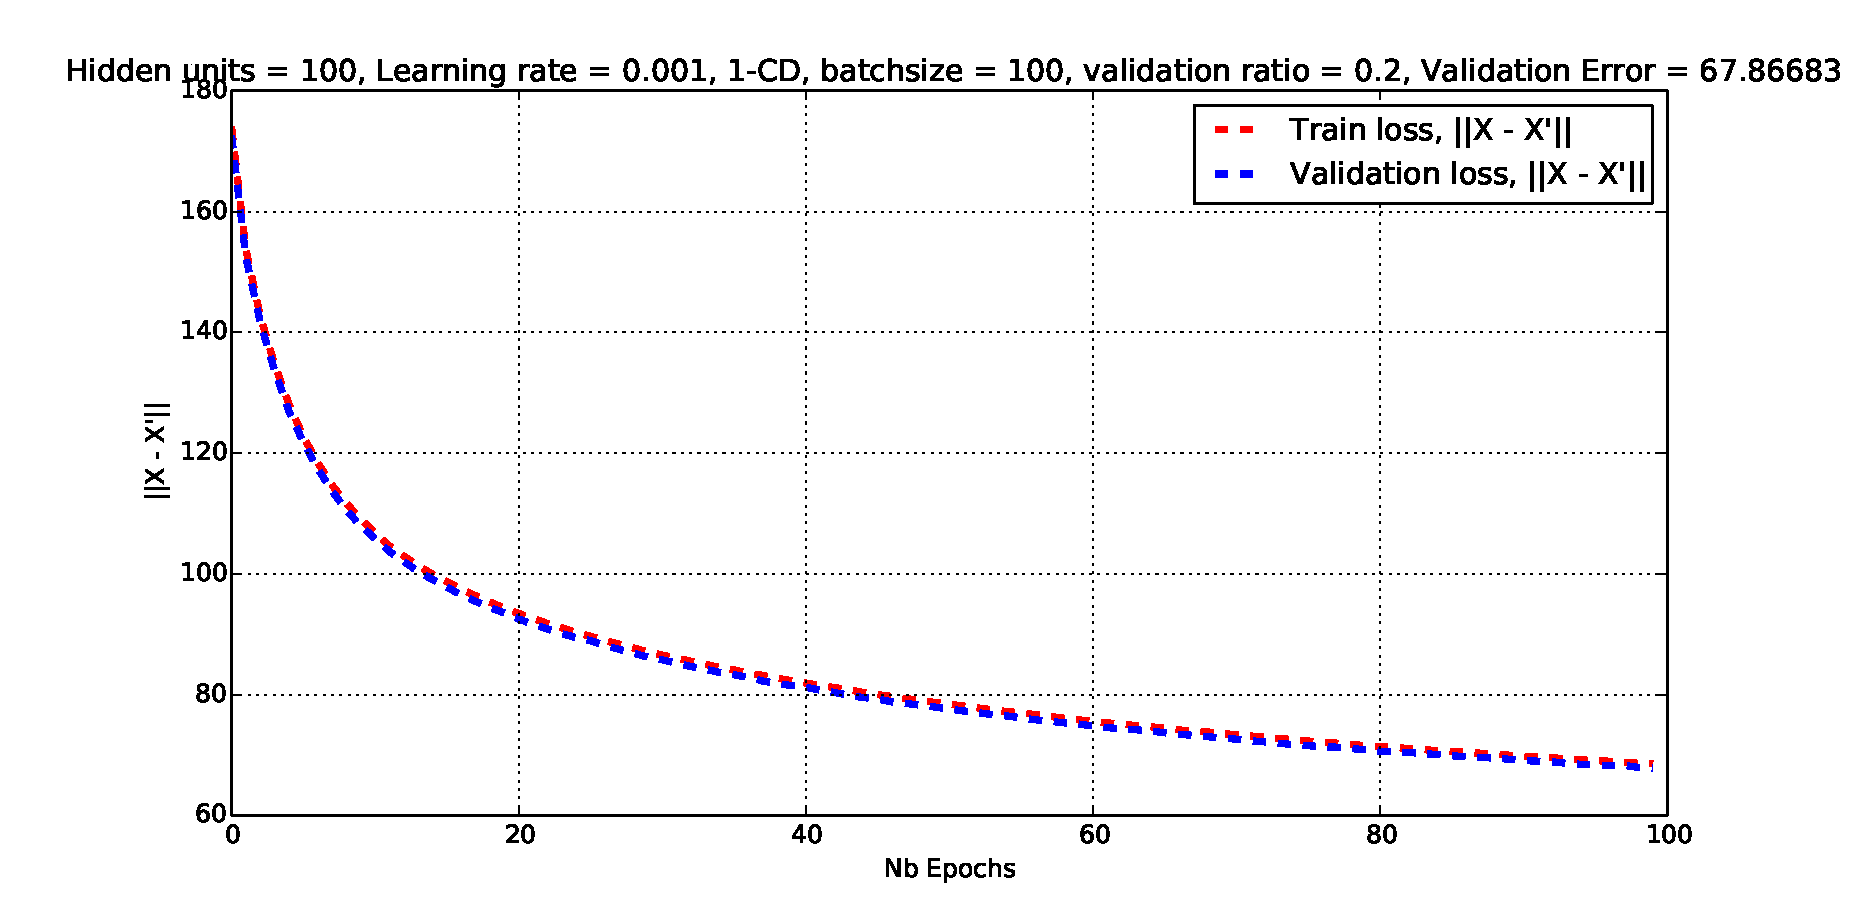
\includegraphics[width=\linewidth]{train_loss}
\captionof{figure}{\smaller Evolution of training loss over epochs}
\end{center}

Generating samples from the learned distribution gives us the following reconstruction images shown in figure 2.
\begin{center}
    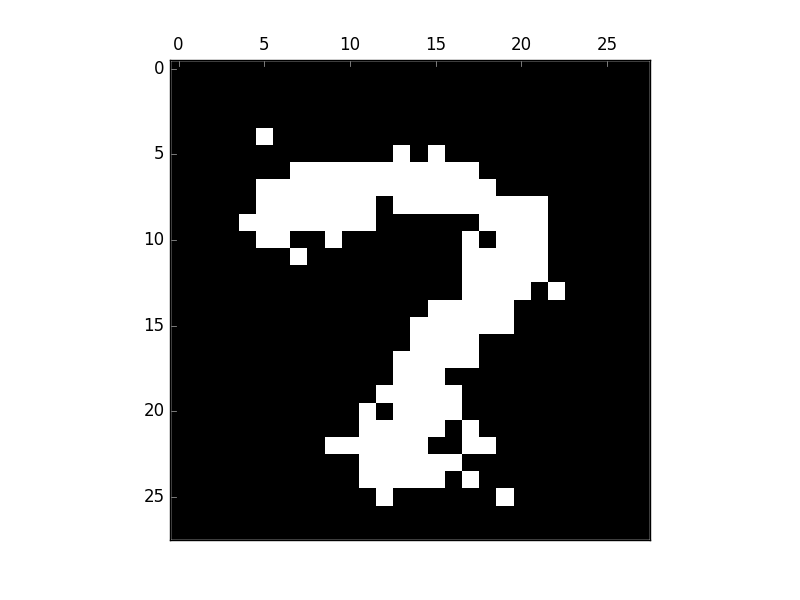
\includegraphics[width=0.15\linewidth]{sample0_at_epoch100}
    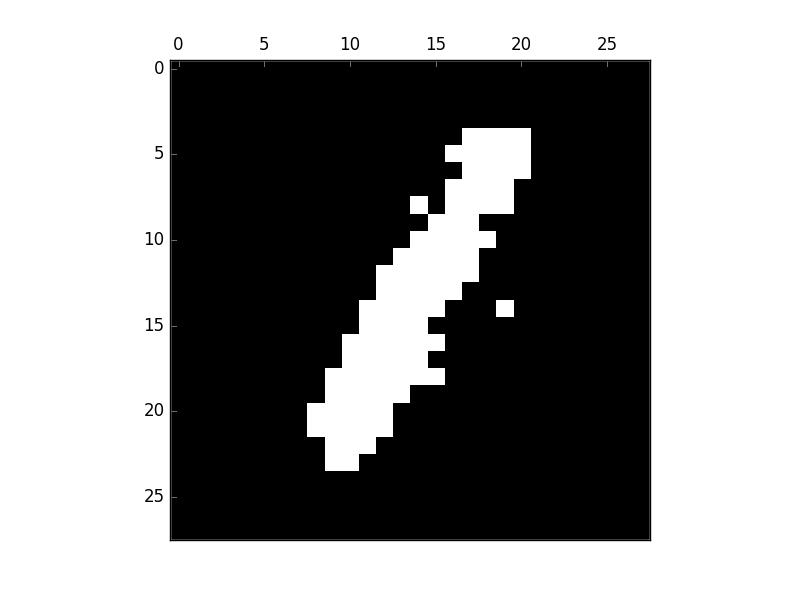
\includegraphics[width=0.15\linewidth]{sample2764_at_epoch100}
    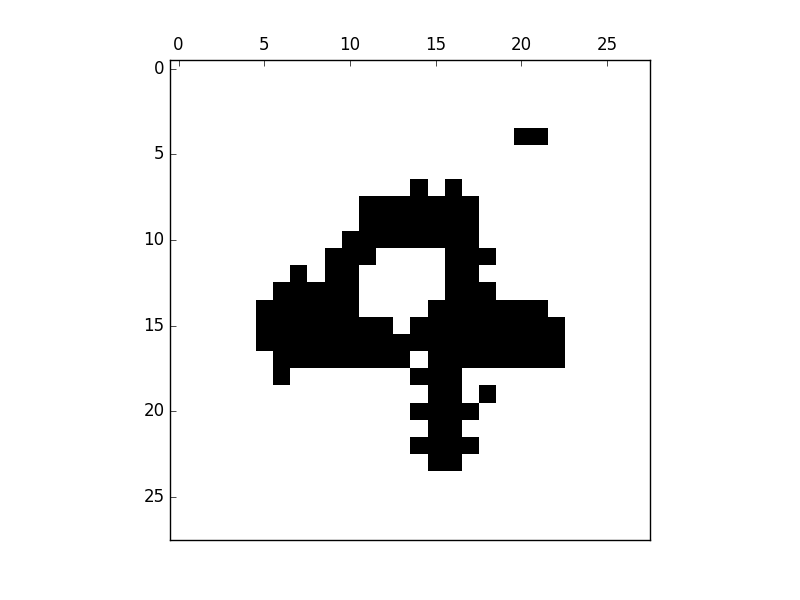
\includegraphics[width=0.15\linewidth]{sample31227_at_epoch100}
    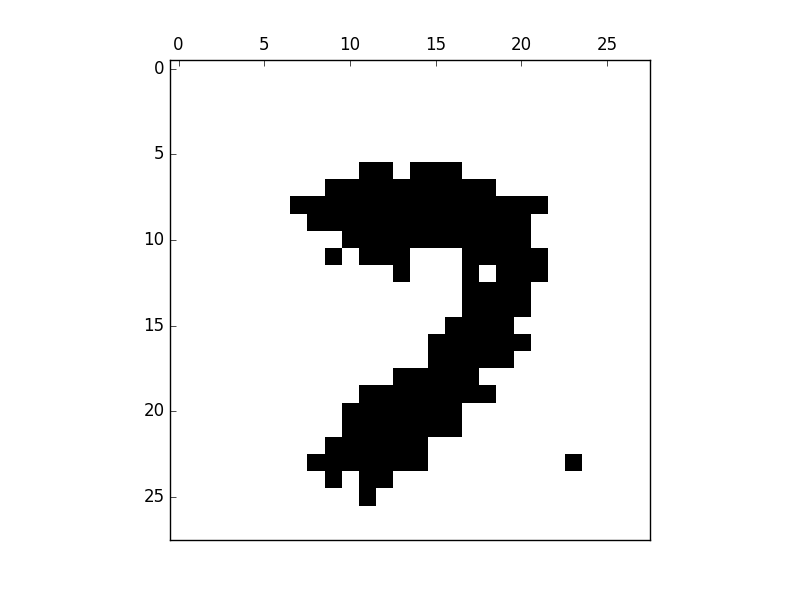
\includegraphics[width=0.15\linewidth]{sample44983_at_epoch100}
    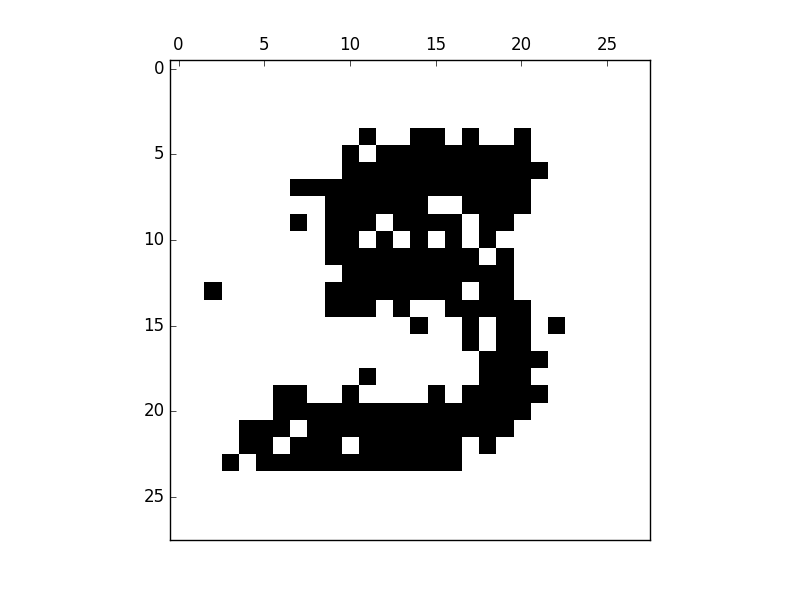
\includegraphics[width=0.15\linewidth]{sample72_at_epoch100}
    \captionof{figure}{\smaller Generated samples after 20 epochs}
\end{center}

The figure 3 is the visualization of the extracted features.

\begin{center}
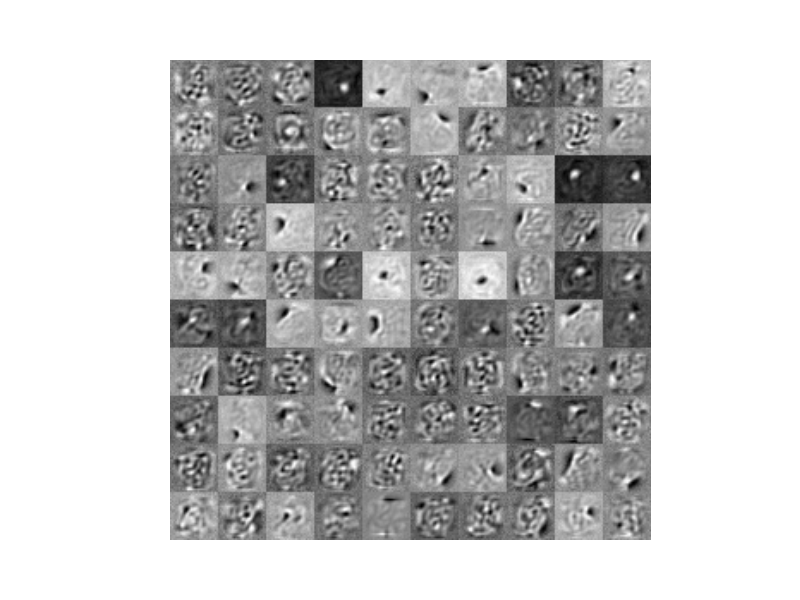
\includegraphics[width=0.4\linewidth]{MNIST_Filter_20Epochs}
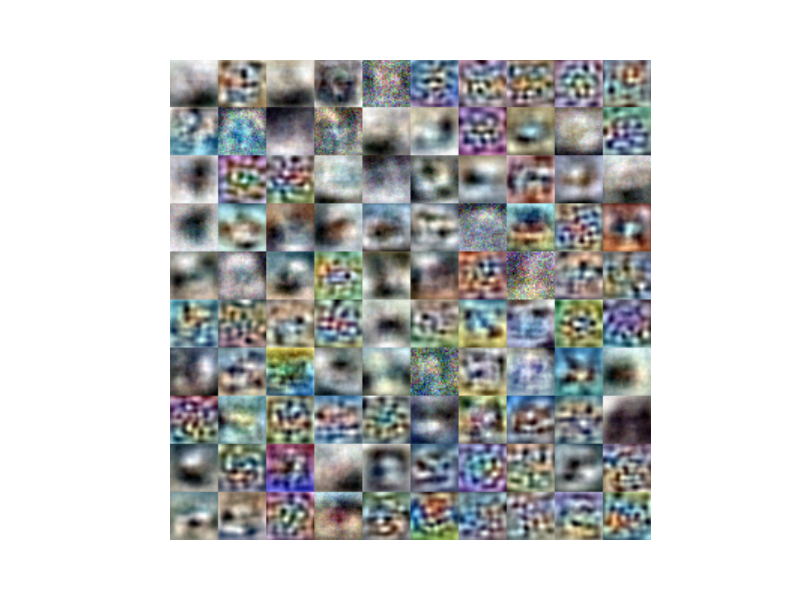
\includegraphics[width=0.4\linewidth]{CIFAR_LearnedWeights}
\captionof{figure}{\smaller Extracted features after 20 Epochs, left: MNIST, right: CIFAR}
\end{center}

In order to understand the influence of parameters involved in RBM training, we compare the evolution of the reconstruction loss over epochs of different batch sizes (figure 4) and different number of hidden units (figure 5) and different number of contrastive divergence steps.\\

\textbf{Batch size influence}
\begin{center}
	\centering
	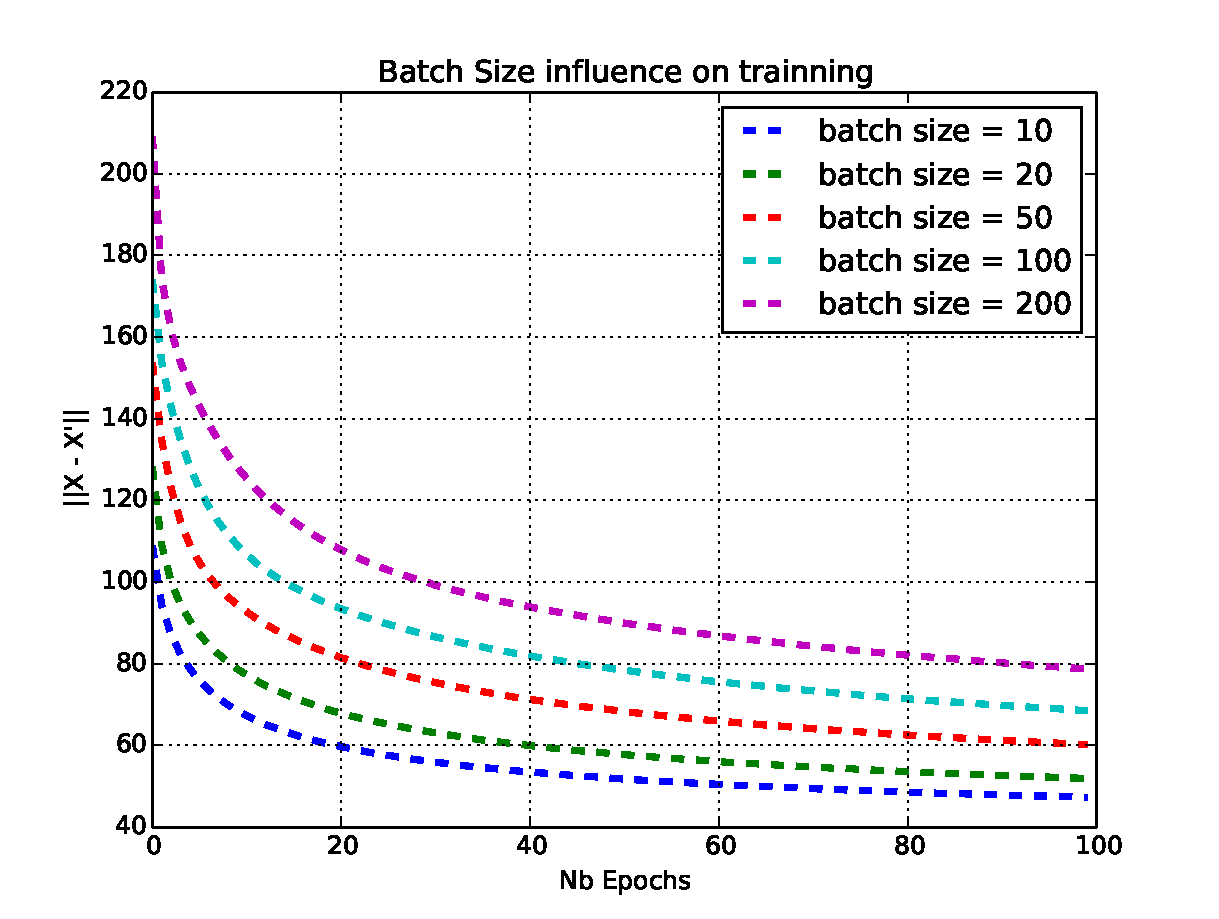
\includegraphics[width=\linewidth,height=0.65\linewidth]{batchsize}
	\captionof{figure}{\smaller Reconstruction loss with 100 hidden units and varying batch size}
\end{center}

Small batch size achieves smaller reconstruction loss. \\
% Increasing the number of hidden units improves the performance but the risk of overfitting increases. We found that about 250 hidden layers is a good trade-off for the MNIST and CIFAR datasets.

\textbf{Number of hidden units influence}
\begin{center}
	\centering
	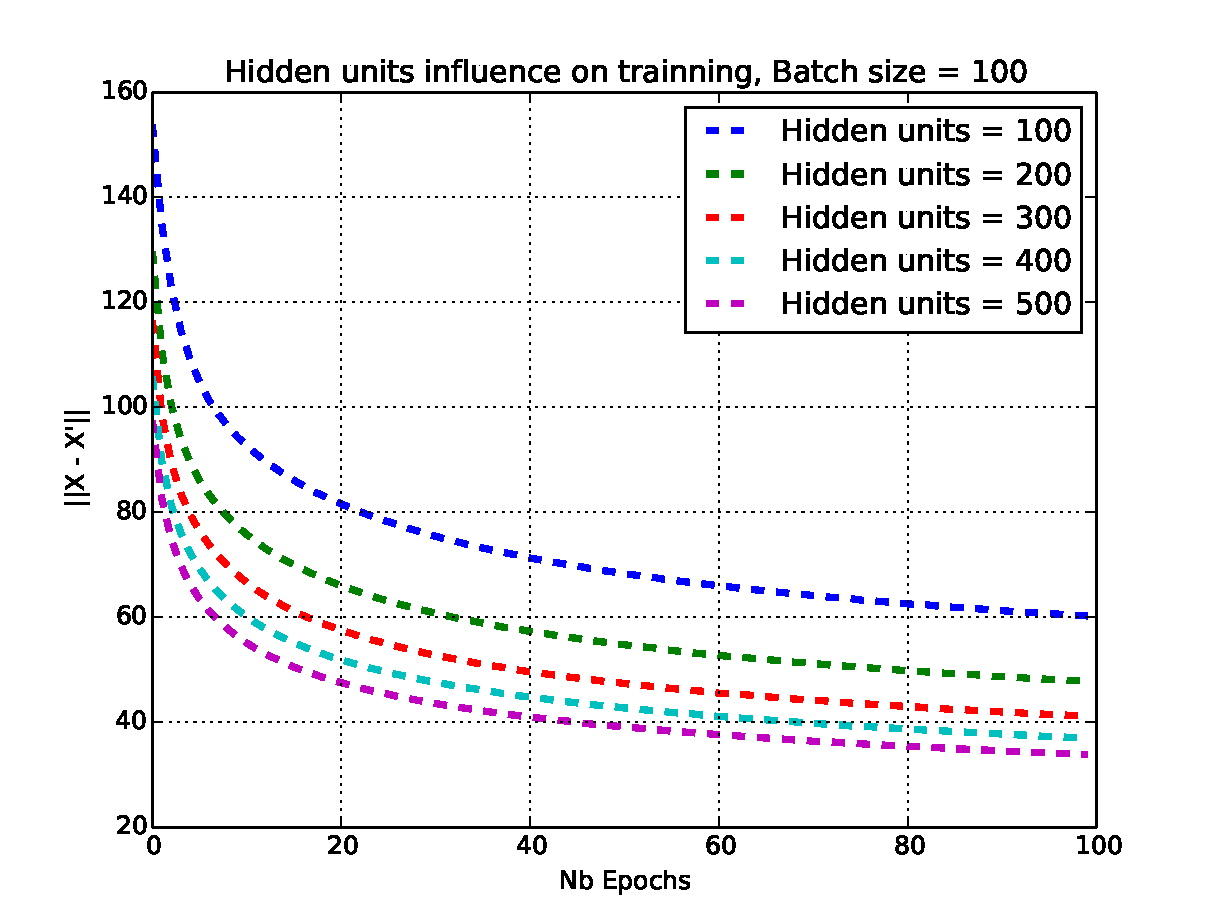
\includegraphics[width=\linewidth,height=0.65\linewidth]{hidden_units}
	\captionof{figure}{\smaller Reconstruction loss with varying number of hidden units}
\end{center}
Increasing the number of hidden units improves the training performance but rises computation time, 250 hidden units is a good choice for MNIST and CIFAR data. 

\end{multicols}

}




%----------------------------------------------------------------------------------------

\end{poster}

\end{document}